%%%%%%%%%%%%%%%%%%%%%%%%%%%%%%%%%%%%%%%%%%%%%%%%%%%%%%%%%%%%%%%%%%%%%%%%%%%%%%%%%%%%%%%
%%%%%%%%%%%%%%%%%%%%%%%%%%%%%%%%%%%%%%%%%%%%%%%%%%%%%%%%%%%%%%%%%%%%%%%%%%%%%%%%%%%%%%%
%%%%%%%%%%%%%%%%%%%%%%%%%%%%%%%%%%%%%%%%%%%%%%%%%%%%%%%%%%%%%%%%%%%%%%%%%%%%%%%%%%%%%%%
\section{ Solução da equação $\DTVECTOR{x}(t) + \MATRIX{P} \VECTOR{x}(t)=0$ }

\begin{theorem}[Equação 
$\DTVECTOR{x}(t) + \MATRIX{P} \VECTOR{x}(t)=0$ com matriz $\MATRIX{P}$ diagonalizável:]
\label{theo:differential-eq:order1:0}
Dados o vetor coluna $\VECTOR{x} \in \mathbb{R}^N$, 
a \hyperref[def:diagonalization0]{\textbf{matriz diagonalizável}} $\MATRIX{P} \in \mathbb{R}^{N\times N}$,
com $N$ autovalores $\lambda_n$ e seus correspondentes autovetores $\VECTOR{v}_n$,
$\forall n \in \{1, 2, ..., N\}$, 
e definida a equação diferencial matricial,
\begin{equation}
\DTVECTOR{x}(t) + \MATRIX{P} \VECTOR{x}(t)=0.
\end{equation}
A solução\footnote{A
demonstração pode ser vista na Prova \ref{proof:theo:differential-eq:order1:0}.} dessa equação diferencial tem  a forma,
\begin{equation}\label{eq:theo:firstorder:2}
 \VECTOR{x}(t)= \MATRIX{V}\MATRIX{D} e^{-\VECTOR{a}t}
\end{equation}
\begin{itemize}
\item \textbf{Desconhecidos:} A matriz diagonal $\MATRIX{D} \in \mathbb{R}^{N \times N}$, e
\item  \textbf{Conhecidos:} São definidos $\MATRIX{V}=
\begin{bmatrix}
\VECTOR{v}_1 & \VECTOR{v}_2 & \dots & \VECTOR{v}_N
\end{bmatrix}$, 
$\VECTOR{a}=
\begin{bmatrix}
\lambda_1 & \lambda_2 & \dots & \lambda_N
\end{bmatrix}^{\transpose}$.
\end{itemize}
\end{theorem}

\begin{corollary}[Forma alternativa da solução do Teorema \ref{theo:differential-eq:order1:0}:]
\label{coro:differential-eq:order1:0}
Outra forma de escrever a Eq. (\ref{eq:theo:firstorder:2}) é usando $\MATRIX{D}=\funcdiag(\VECTOR{d})$, de modo que
\begin{equation}\label{eq:coro:firstorder:1}
 \VECTOR{x}(t)= \MATRIX{V}~\funcdiag(e^{-\VECTOR{a}t})~\VECTOR{d}.
\end{equation}
\end{corollary}

\begin{corollary}[Calculando $\MATRIX{D}$ desde $\VECTOR{x}(t_1)$ na solução do Teorema \ref{theo:differential-eq:order1:0}:]
\label{coro:differential-eq:order1:1}
Conhecidos a Eq. (\ref{eq:theo:firstorder:2}) e o Corolário \ref{coro:differential-eq:order1:0},
podemos calcular
$\MATRIX{D}=\funcdiag(\VECTOR{d})$ 
usando os dados $\VECTOR{x}(t_1)$, de modo que
\begin{equation}\label{eq:coro:differential-eq:order1:1:a}
\VECTOR{d} =
\left[ \MATRIX{V}~\funcdiag(e^{-\VECTOR{a}t})~ \right]^{-1}
\VECTOR{x}(t_1).
\end{equation}
\end{corollary}

\begin{corollary}[Calculando $\MATRIX{D}$ desde $\DTVECTOR{x}(t_1)$ na solução do Teorema \ref{theo:differential-eq:order1:0}:]
\label{coro:differential-eq:order1:2}
Conhecidos a Eq. (\ref{eq:theo:firstorder:2}) e o Corolário \ref{coro:differential-eq:order1:0},
podemos calcular
$\MATRIX{D}=\funcdiag(\VECTOR{d})$ 
usando os dados em $\DTVECTOR{x}(t_1)$, de modo que
\begin{equation}\label{eq:coro:differential-eq:order1:1:b}
\VECTOR{d} =
\left[ -\MATRIX{V}\MATRIX{A}~\funcdiag(e^{-\VECTOR{a}t})~ \right]^{-1}
\DTVECTOR{x}(t_1).
\end{equation}
\end{corollary}

%%%%%%%%%%%%%%%%%%%%%%%%%%%%%%%%%%%%%%%%%%%%%%%%%%%%%%%%%%%%%%%%%%%%%%%%%%%%%%%%
\subsection{Exemplos da solução da equação $\DTVECTOR{x}(t) + \MATRIX{P} \VECTOR{x}(t)=0$}

\begin{example}[Procurando a resposta 
$\VECTOR{x}(t)$ usando o Teorema \ref{theo:differential-eq:order1:0}:]
\label{ex:dxPx:0}
Calcular o vetor $\VECTOR{x}(t)$,
conhecida a equação diferencial, $\DTVECTOR{x}(t) + \MATRIX{P} \VECTOR{x}(t)=0$, com 
um vetor $\VECTOR{x} \in \mathbb{R}^{N}$, uma matriz $\MATRIX{P}$ e a amostras em $\VECTOR{x}(0)$,
\begin{equation}
\MATRIX{P}=
\begin{bmatrix}
3 & -2 & 0\\
-2 & 3 & -1\\
0 & -1 & 1
\end{bmatrix}
\qquad \wedge \qquad
\VECTOR{x}(0)=
\begin{bmatrix}
0\\
0\\
1
\end{bmatrix}.
\end{equation}
\end{example}



\begin{SolutionT}[Relativa ao Exemplo \ref{ex:dxPx:0}:]
\label{ex:dxPx:0:sol1}
Dado que a matriz $\MATRIX{P}$ é simétrica, e
sabendo que $\lambda_{\MATRIX{P}}$ e $\MATRIX{V}$ são matrizes correspondentes aos autovalores e os autovetores de $\MATRIX{P}$,
respetivamente; 
\begin{equation}
\lambda_{\MATRIX{P}}=
\begin{bmatrix}
   0.23844 &       0 &       0\\
         0 & 1.63667 &       0\\
         0 &       0 & 5.12489
\end{bmatrix}
\quad \wedge \quad
\MATRIX{V}=
\begin{bmatrix}
  -0.40181 & 0.61887 &-0.67495\\
  -0.55481 & 0.42186 & 0.71709\\
  -0.72852 &-0.66260 &-0.17385
\end{bmatrix}.
\end{equation}
podemos usar o Teorema \ref{theo:positivematrix1} para declarar que a matriz $\MATRIX{P}$ é diagonalizável. 
Assim, da Eq. (\ref{eq:coro:differential-eq:order1:1:a}) do Corolário \ref{coro:differential-eq:order1:1},
obtemos
\begin{equation}
\VECTOR{d}=
\begin{bmatrix}
  -0.72852\\
  -0.66260\\
  -0.17385
\end{bmatrix}
\end{equation}
de modo que se identificarmos $\VECTOR{a}=[0.23844~ 1.63667~ 5.12489]^{\transpose}$ 
como a diagonal de $\lambda_{\MATRIX{P}}$,
obtemos
\begin{equation}
 \VECTOR{x}(t)= 
\begin{bmatrix}
   0.292724 &-0.410061 & 0.117337\\
   0.404188 &-0.279524 &-0.124664\\
   0.530738 & 0.439039 & 0.030222
\end{bmatrix}
\begin{bmatrix}
   e^{-0.23844 t}\\
   e^{-1.63667 t}\\
   e^{-5.12489 t}
\end{bmatrix},
\end{equation}
a Figura \ref{fig:ex:dxPx:0} mostra um gráfico do vetor $\VECTOR{x}(t)$.
\end{SolutionT}
     \begin{figure}[!h]
         \centering
         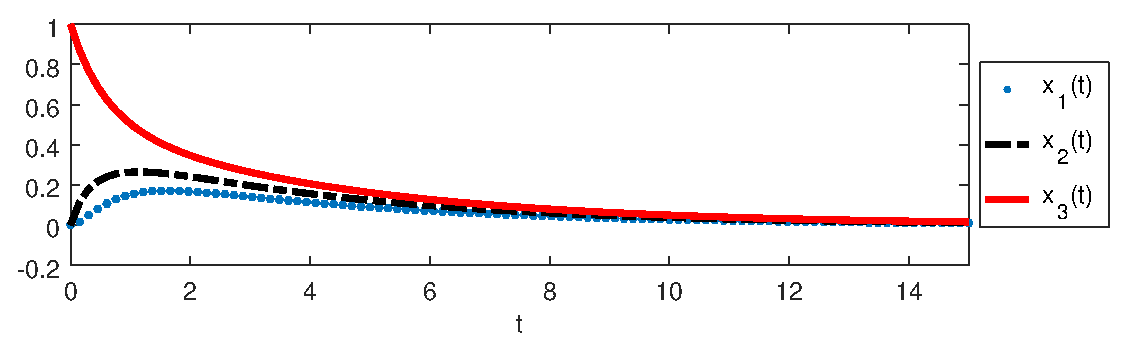
\includegraphics[width=0.99\textwidth]{chapters/differential-eq/mfiles/primeiroorder/primeirooder1.eps}
         \caption{Resposta $\VECTOR{x}(t)$ do Exemplo \ref{ex:ddxPx:0}.}
         \label{fig:ex:dxPx:0}
     \end{figure}
